\begin{figure}[t]
    \centering
    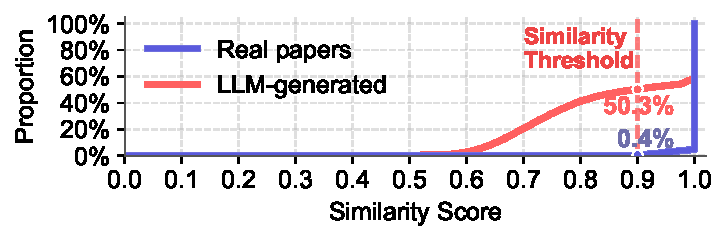
\includegraphics[width=\columnwidth]{Sec3_Methodology/llm_papers_similarity_ecdf.pdf}
    \vspace{-5.5mm}
\caption{ECDF of title similarity scores: LLM-generated vs.\ real-paper citations.}
    \label{fig:llm_papers_similarity_ecdf}
\end{figure}

%%%%%%%%%%%%%%%%%%%%%%%%%%%%%%%%%%%%%%%%%%%%%%%%%%%%%%%%%%%%%%%%%%%%%%%%%%%%%%%%
% JUSTIFICATION FOR DIFFERENTIAL THRESHOLDING IN CITATION VALIDATION
% ------------------------------------------------------------------------------
% This section provides the statistical rationale for applying a Similarity 
% Threshold of 1.0 for LLM-generated citations versus 0.9 for Real Papers.
%%%%%%%%%%%%%%%%%%%%%%%%%%%%%%%%%%%%%%%%%%%%%%%%%%%%%%%%%%%%%%%%%%%%%%%%%%%%%%%%

% 1. VALIDATION OF REAL PAPER THRESHOLD (Threshold = 0.9)
% ------------------------------------------------------------------------------
% Observation: The ECDF of 'Real papers' (green line) remains near zero until 
% reaching the [0.9, 1.0] interval, with a value of only 0.4% at x = 0.9.
%
% Rationale: 
% - The steep vertical jump at x > 0.9 indicates that 99.6% of real citations 
%   exhibit high fidelity to the ground truth.
% - The delta between 0.9 and 1.0 is categorized as 'Measurement Noise' 
%   (e.g., OCR character recognition errors, hyphenation, or minor typos).
% - Thus, 0.9 is a robust boundary that ensures high Recall by accommodating 
%   non-systematic technical artifacts without sacrificing validity.

% 2. VALIDATION OF LLM-GENERATED THRESHOLD (Threshold = 1.0)
% ------------------------------------------------------------------------------
% Observation: The ECDF of 'LLM-generated' (blue line) exhibits a gradual 
% slope starting from x = 0.6, with a cumulative value of ~54.1% at x < 1.0.
%
% Rationale: 
% - Unlike real papers, LLMs exhibit 'Structural Bias' rather than random noise.
% - The high density of citations in the [0.6, 0.99] range represents 
%   'Near-miss Hallucinations'—citations that appear semantically plausible 
%   but are factually non-existent or logically spliced.
% - Adopting a strict Exact Match (Similarity = 1.0) is mandatory to ensure 
%   High Precision, filtering out sophisticated hallucinations that would 
%   otherwise pass a 0.9 threshold.

% 3. STATISTICAL CONCLUSION
% ------------------------------------------------------------------------------
% The divergence between the quasi-binary distribution of Real Papers and the 
% continuous dispersion of LLM outputs justifies the use of an asymmetric 
% decision boundary. This prevents the inflation of LLM accuracy while 
% maintaining the empirical verifiability of human-authored research.
%%%%%%%%%%%%%%%%%%%%%%%%%%%%%%%%%%%%%%%%%%%%%%%%%%%%%%%%%%%%%%%%%%%%%%%%%%%%%%%%
